
\chapter{Layered Stigmergy}
\label{chap:lay_stig}

This chapter will outline the implementation of a multi layered stigmergy algorithm, as an attempt to create a swarm algorithm which better avoids collision than simple 1 layered stigmergy. The algorithm implemented in this chapter is identical to the Stigmergy algorithm from Chapter \ref{chap:stigmergy}, in the way that it used the same pheromone grid to navigate its agents. It also uses the same reaction to the pheromones, and the same rules for placement. 

The difference will be that this algorithm contains 2 pheromone grids instead of a single one.

\subsection{Assumptions}
Having two pheromone grids implies the assumption that the agents are able to tell two different kind of pheromones apart. Digitally this is represented as two different grids, but the effect is assumed also be achievable with a multitude of different concentration levels in a single pheromone grid, as long as the agents can differentiate between the concentrations. 


\subsection{Specifications}
Table \ref{tab:vars_12} shows the specifications of the second pheromone grid. Note that the specifications of the other pheromone grid is identical to one from previous chapter, along with the rest of the algorithm as well.

\begin{table}[H]
\centering
\begin{tabularx}{0.6\textwidth}{ll}
\toprule
\textbf{Variables}     & \textbf{Value}  \\ \hline
Pheromone grid size    & $30 \times 10 \times 10$ \\ \hline
Pheromone fatigue      & $2/s$               \\
Number of pheromone grids      & $2$               \\
Constant pheromone  & $2$             \\
Triggered pheromone & $0$               \\
\end{tabularx}
\caption{Specifications of 2nd pheromone grid}
\label{tab:vars_12}
\end{table}

\begin{itemize}
\item{The \textbf{Pheromone grid} is similar in size to the first pheromone grid}
\item{\textbf{Pheromone fatigue} is high in the second grid, meaning that a pheromone will disappear approximately 1 second after it has been placed}
\item{This second grid only operates with \textbf{Constant pheromones} in contrast to the first. This means that the agents always trail pheromones after them on this grid, but to not change the strength of their pheromone based on outside events}
\item{\textbf{Number of pheromone grids} is now 2, hence the name \textit{layered stigmergy} as there are more layers/kinds of pheromones}
\end{itemize}

\subsection{Development of pheromones in 2nd layer}
The aim of the 2nd layer of pheromones, is to enable the agents to tell each other apart and evaluate a distance or direction to other agents. As such the pheromones disappear quickly after being placed, but have very simple rules. The only condition for placement of a pheromone in the second layer, is that an agent is at the same location as the pheromone being placed.

\subsection{Reacting to Pheromones}
The agents have been given the added condition, that any area they move into, must not have a pheromone in the second layer. As such, if there is a digital marker in the second grid at a position, an agent cannot be in that position. If the agent has itself placed the marker, the check happens before the placement, to avoid agents moving away from themselves. 

When a marker near is detected in the 2nd, a search is recalculated based on the pheromones in the 1st grid.

\section{Testing}
\label{chap:stigmergy_test}

\subsection{Pheromone grids}
The resulting pheromone grids from running the simulation are updated throughout the simulation. Figure \ref{fig:sources} shows the 2nd layer of pheromones, which approximately denotes the agent positions. The faster the pheromones decay the more accurately the pheromones display the positions of the agents. From the position of the pheromones in the grid, it can be seen that they are not colliding.

% Pheromones
\begin{figure}[H]
	\centering
	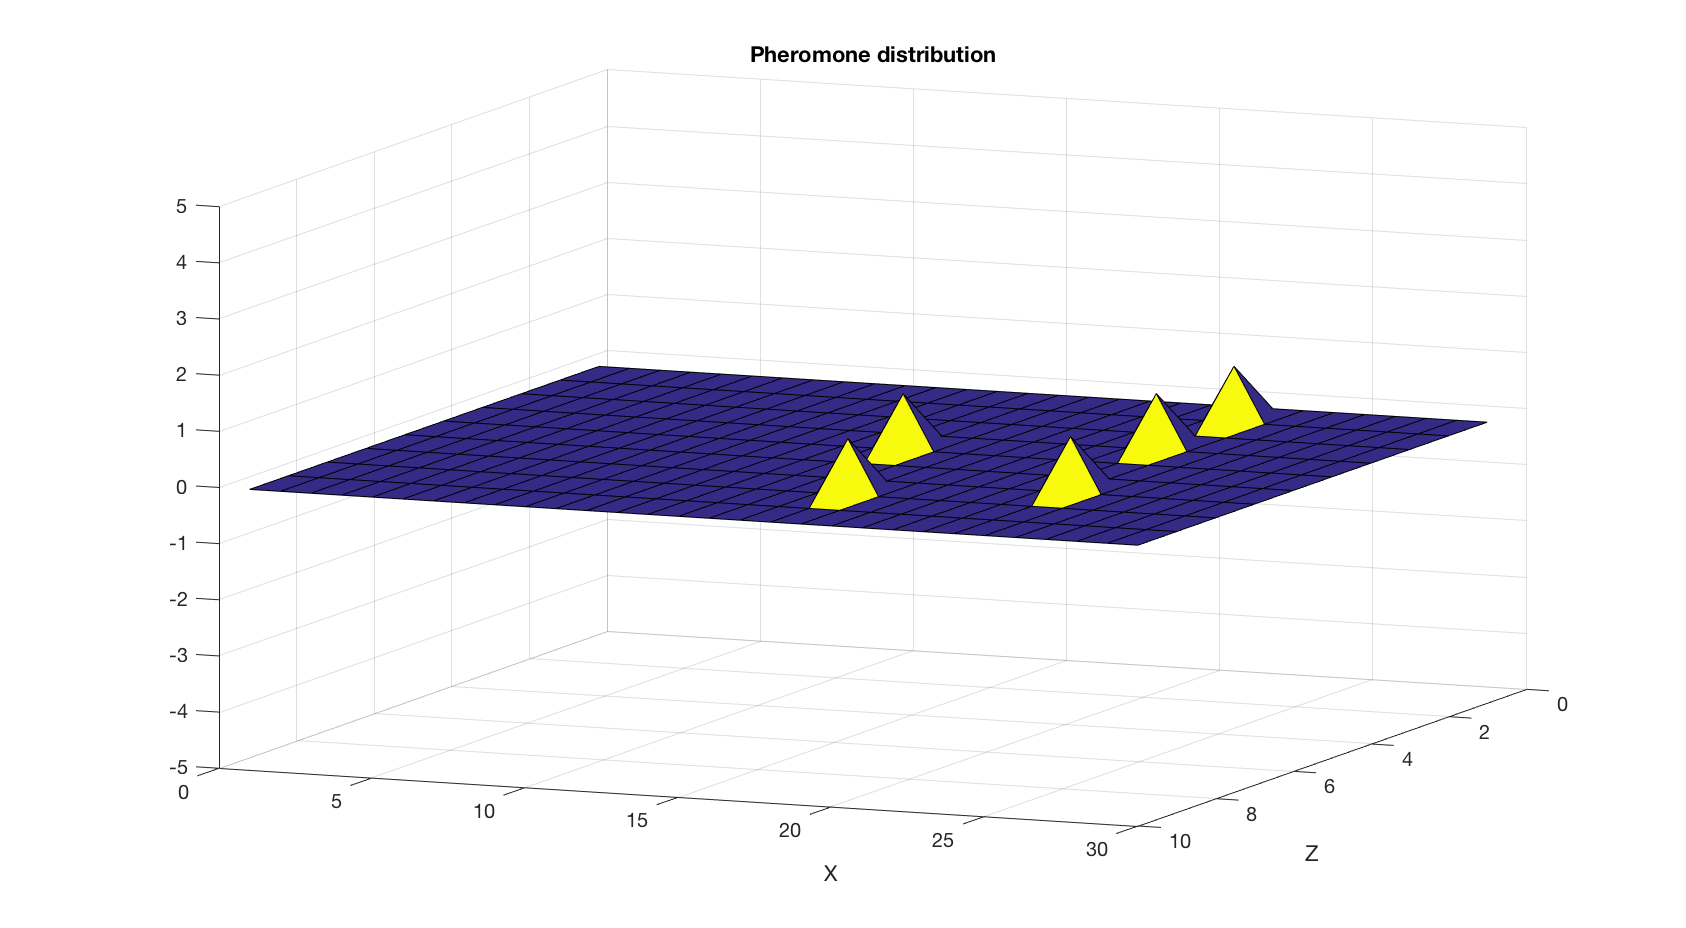
\includegraphics[width=1\columnwidth]{figures/STIG_source_pheromones}
  	\caption{\label{fig:sources}2nd Pheromone layer (Pheromone sources) snapshot from simulation}
\end{figure}

The 1st pheromone grid, is roughly similar to grid from previous implementation, as it can be seen in Figure \ref{fig:phero_post1}.

% Pheromones
\begin{figure}[H]
	\centering
	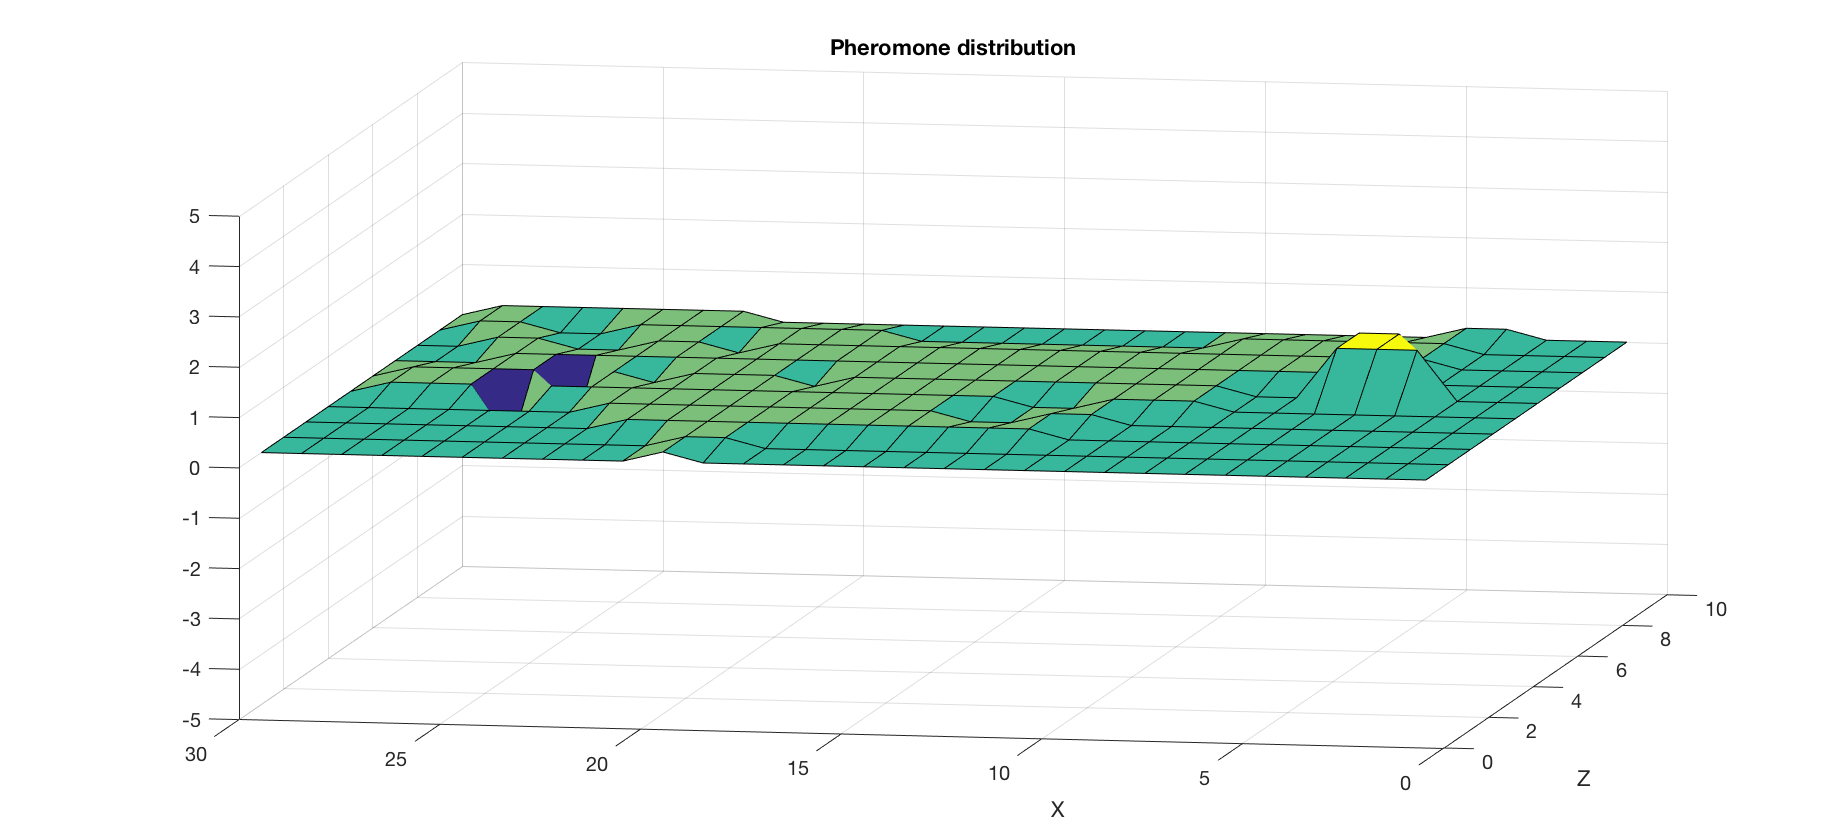
\includegraphics[width=1\columnwidth]{figures/STIG_lay_grid1}
  	\caption{\label{fig:phero_post2}1st pheromone grid after simulation has finished (mapped onto the horizontal dimensions)} 
\end{figure}

\subsection{Performance}

The overall performance results of the layered stigmergy algorithm can be found in Figure \ref{tab:stig_metrics_lay}.

% Environment Specifications
\begin{table}[H]
\centering
\begin{tabularx}{1\textwidth}{l@{ }Xr}
\toprule
\textbf{Metric} &\textbf{Preference} & \textbf{Kind} \\ \midrule
Number of collisions  & Lowest & $23$  \\
Time spent completing control problem & Lowest & $242.8 seconds$  \\
Utility of space & Lowest & $78\%$  \\
Shape of flight pattern  & N/A & See comments below \\
\bottomrule
\end{tabularx}
\caption{Layered Stigmergy performance}
\label{tab:stig_metrics_lay}
\end{table}

\begin{itemize}
\item{\textbf{Number of collisions} - The aim of implementing a second pheromone layer, was to decrease the number of collision. This was unsuccessful, however the time spent in a collision is a lot lower than in the non-layered stigmergy algorithm. As such, the layered stigmergy can be seen to have a positive impact in the fact that the agent move away from each other when colliding. }
\item{\textbf{Time spend completing the control problem} - With over a doubling in the simulation time, it is possible to argue that the benefit of lower collision time, is worth the efficiency drawback}
\item{\textbf{Utility of space} - 4\% higher than the non-layered stigmergy algorithm, can be considered a fine result, since the collision avoidance requires more space to maneuver within}
\item{\textbf{Shape of flight pattern} - The flight pattern is very similar to the flight pattern on the non-layered stigmergy algorithm. The difference is when agents attempt to avoid a collision, and spend a long time moving in the opposite direction of their desired location. This result is due to the fact that there is no optimization to the collision avoidance. As such, when avoiding a collision, an agent is simple reattempting a search in a different direction, as it normally would as a part of the swarm}
\end{itemize}

% Pheromones
\begin{figure}[H]
	\centering
	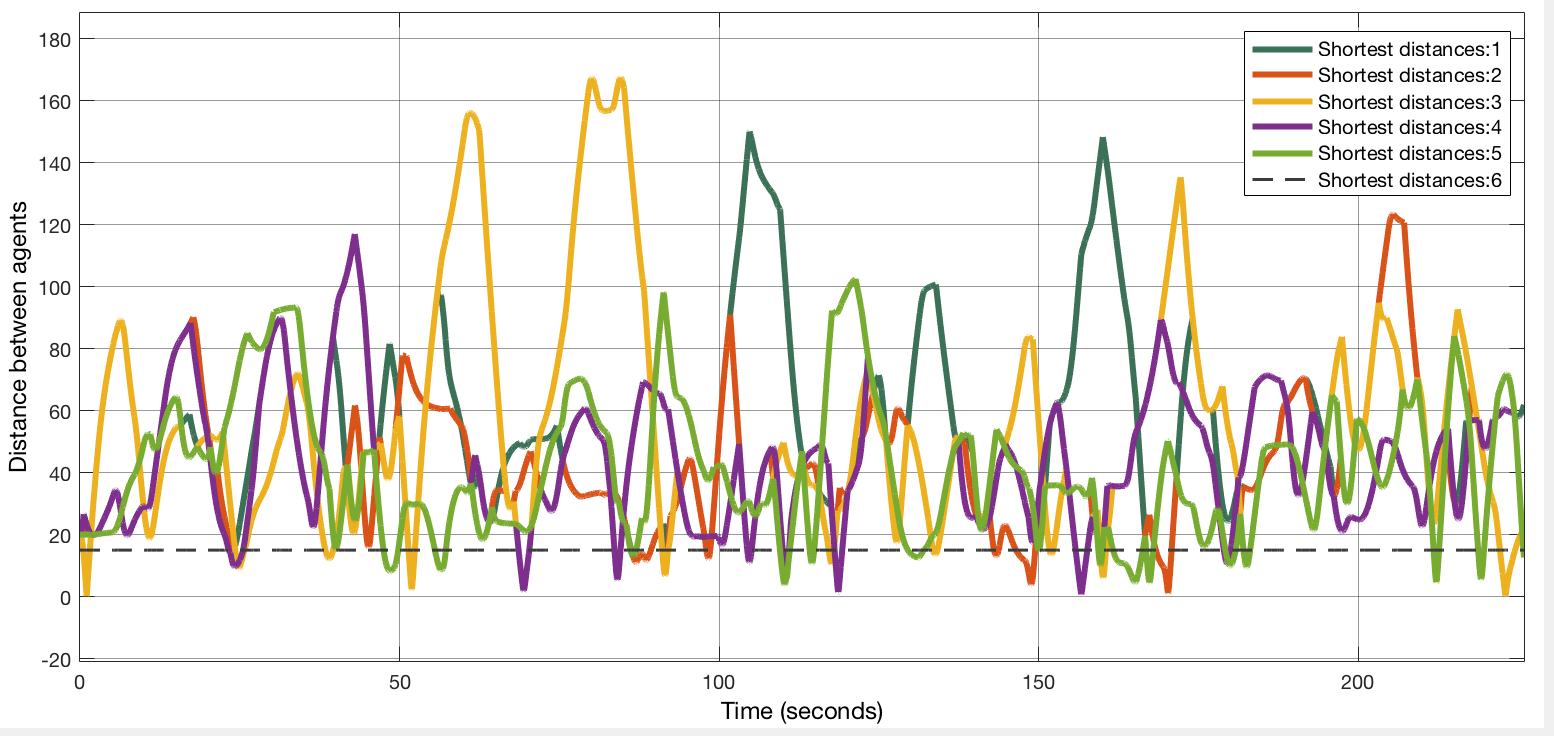
\includegraphics[width=1\columnwidth]{figures/STIG_random_agent_overlap_lay}
  	\caption{\label{fig:3d_stig_solved}Collisions of agents throughout simulation, with layered stigmergy}
\end{figure}

% Pheromones
\begin{figure}[H]
	\centering
	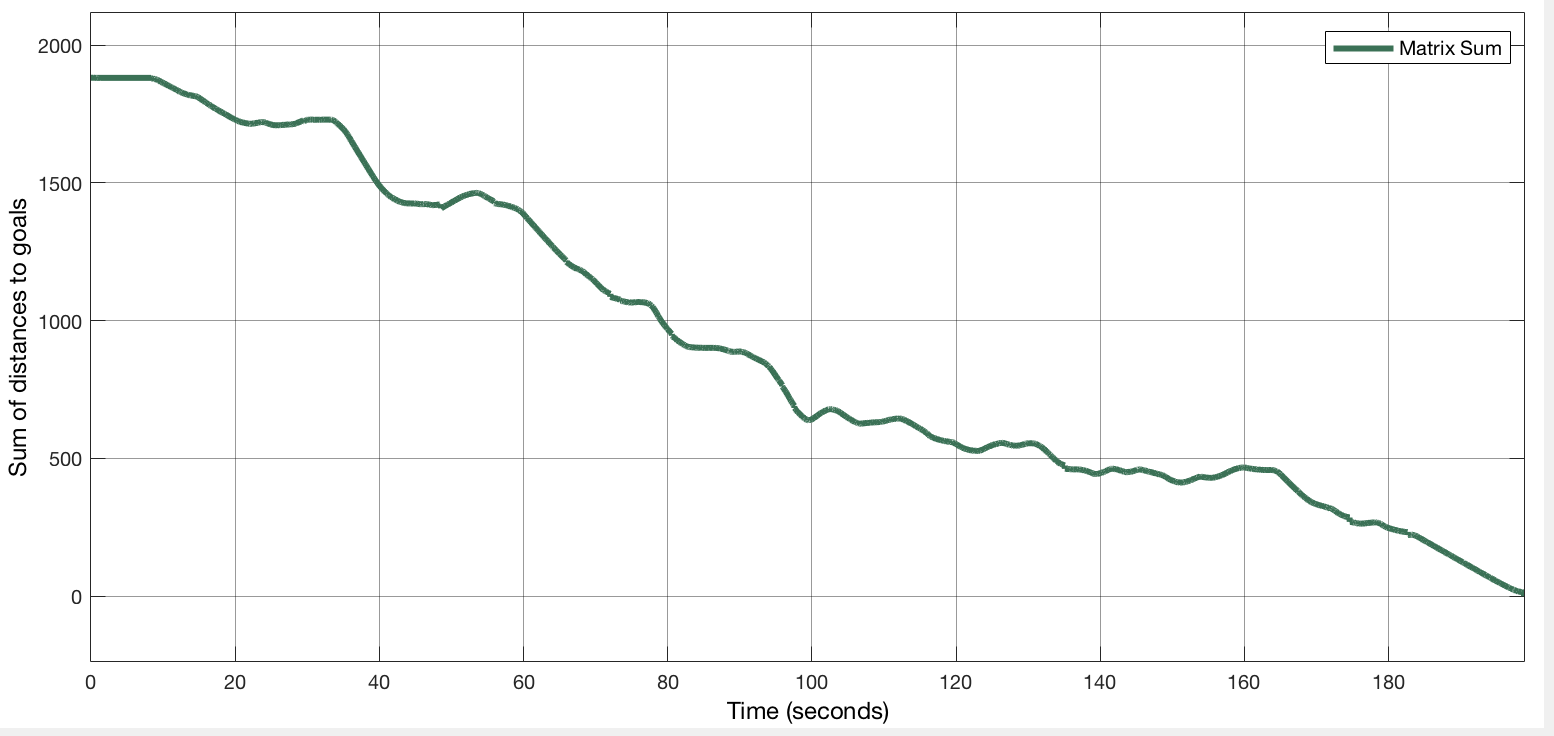
\includegraphics[width=1\columnwidth]{figures/STIG_random_lay}
  	\caption{\label{fig:3d_stig_approx}Total distances for blocks to goals over time}
\end{figure}

\subsection{Improvement}
The improvement over the non-layered stigmergy is only in terms of collision time. On other aspects such as completion time of the control problem and the number of collisions, this implementation using a layered stigmergy strategy, did not yield results good enough safely suggest multiple layers for collision avoidance in stigmergy applications.